\part*{Ejercicio 2}

Se tomaron los datos de m\'aximos y m\'inimos de las entradas y salidas para los distintos estados de las hojas de datos de los circuitos en cuesti\'on, y se exhiben en el cuadro \ref{tab:datos74}.
\begin{table}[H]
\begin{tabular}{|l|l|l|l|l|l|l|}
\hline
                                                                            & Vcc                                                        & Voltage (25 C)                                              & Vcc         & Voltage (25 C) & Vcc      & Voltage (25 C)   \\ \hline
                                                                      & \multicolumn{2}{l|}{74HC02}                                                                                              & \multicolumn{2}{l|}{74HCT02} & \multicolumn{2}{l|}{74LS02} \\ \hline
\begin{tabular}[c]{@{}l@{}}Minimum HIGH Level\\ Input Voltage\end{tabular}  & \begin{tabular}[c]{@{}l@{}}2.0V\\ 4.5V\\ 6.0V\end{tabular} & \begin{tabular}[c]{@{}l@{}}1.5V\\ 3.15V\\ 4.2V\end{tabular} & 4.5V a 5.5V & 2V             & 4.75V    & 2V               \\ \hline
\begin{tabular}[c]{@{}l@{}}Maximum LOW Level\\ Input Voltage\end{tabular}   & \begin{tabular}[c]{@{}l@{}}2.0V\\ 4.5V\\ 6.0V\end{tabular} & \begin{tabular}[c]{@{}l@{}}0.5V\\ 1.35V\\ 1.8V\end{tabular} & 4.5V a 5.5V & 0.8V           & 4.75V    & 0.8V             \\ \hline
\begin{tabular}[c]{@{}l@{}}Minimum HIGH Level\\ Output Voltage\end{tabular} & \begin{tabular}[c]{@{}l@{}}2.0V\\ 4.5V\\ 6.0V\end{tabular} & \begin{tabular}[c]{@{}l@{}}1.9V\\ 4.4V\\ 5.9V\end{tabular}  & 4.5V a 5.5V & 4.4V           & 4.75V    & 2.7V             \\ \hline
\begin{tabular}[c]{@{}l@{}}Maximum LOW Level\\ Output Voltage\end{tabular}  & \begin{tabular}[c]{@{}l@{}}2.0V\\ 4.5V\\ 6.0V\end{tabular} & \begin{tabular}[c]{@{}l@{}}0.1V\\ 0.1V\\ 0.1V\end{tabular}  & 4.5V a 5.5V & 0.1V           & 4.75V    & 0.5V             \\ \hline
\end{tabular}
\caption{Tabla de informaci\'on obtenida de las hojas de datos}
\label{tab:datos74}
\end{table}

Como se ilustra en las figuras para los cuatro casos planteados, s\'olo habr\'ia problemas si se intenta conectar un transistor HC a la salida de un LS: la salida alta del LS puede caer en la regi\'on indeterminada de la entrada del HC, y sin que falle ning\'un componente fallar\'ia el circuito.

En todos los dem\'as casos se genera un margen de error para las entradas de los transistores.

\begin{figure}[H]
\begin{center}
  \begin{minipage}[b]{0.4\textwidth}
  	\begin{center}
  		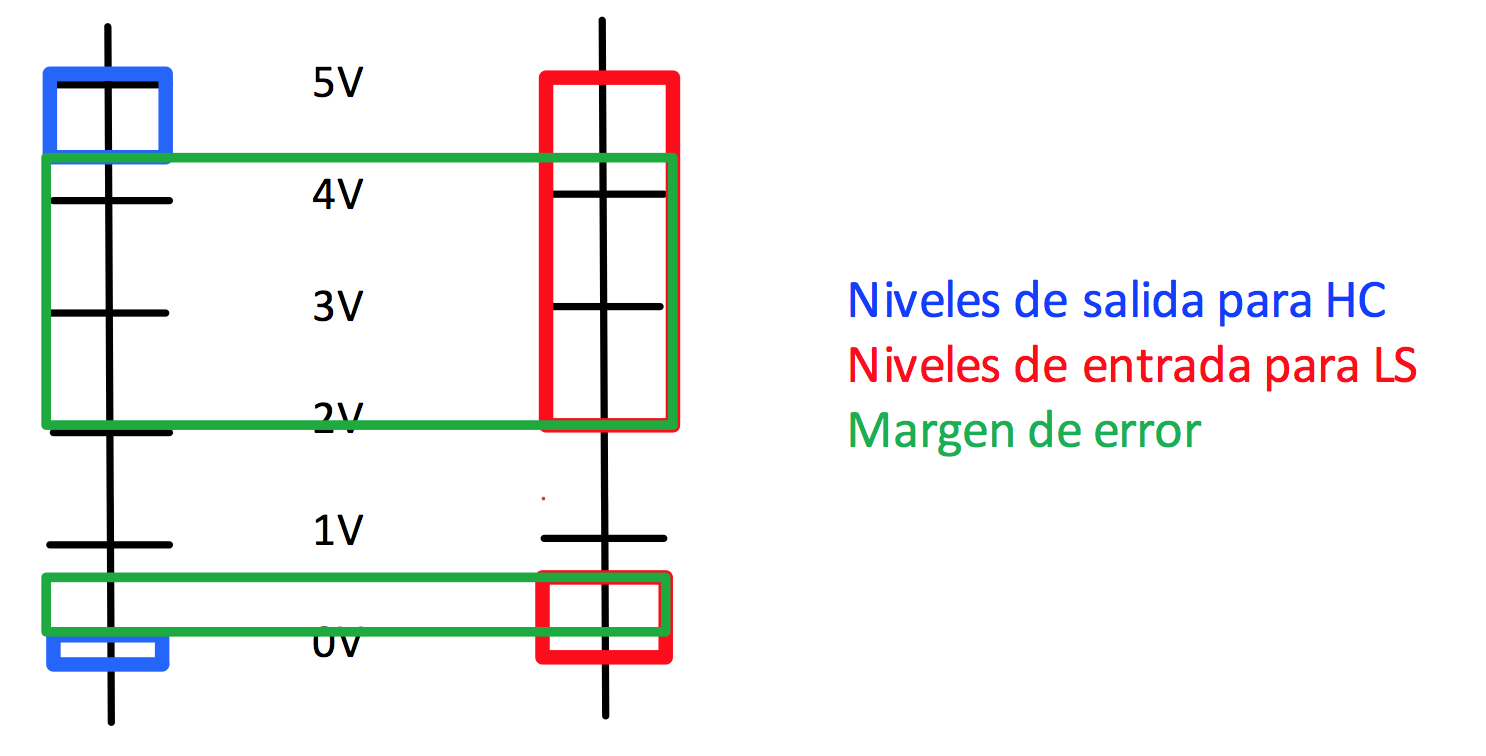
\includegraphics[width=6cm]{ejercicio2/HC-LS}
    \caption{Niveles de tensi\'on para caso HC alimenta a LS.} %caption abajo
  	\end{center}
  \caption{Circuito utilizado}
  \label{7_fig1}
  \end{minipage}
  \begin{minipage}[b]{0.4\textwidth}
    \begin{center}
  		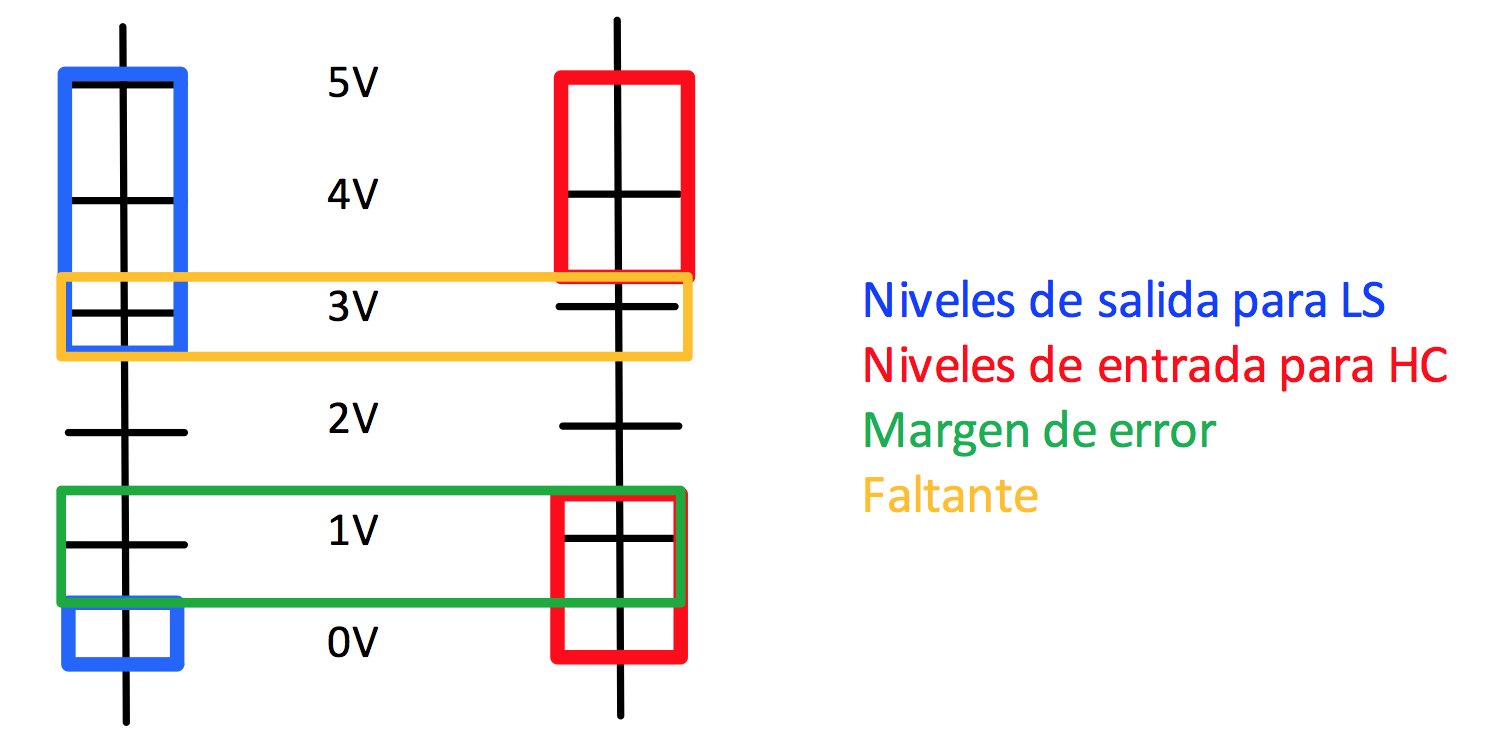
\includegraphics[width=6cm]{ejercicio2/LS-HC}
    \caption{Niveles de tensi\'on para caso LS alimenta a HC.} %caption abajo
	\end{center}
  \caption{Implementaci\'on con 74HC112}
  \label{7_fig2}
 \end{minipage}
\end{center}
\end{figure}


\begin{figure}[H]
\begin{center}
  \begin{minipage}[b]{0.4\textwidth}
  	\begin{center}
  		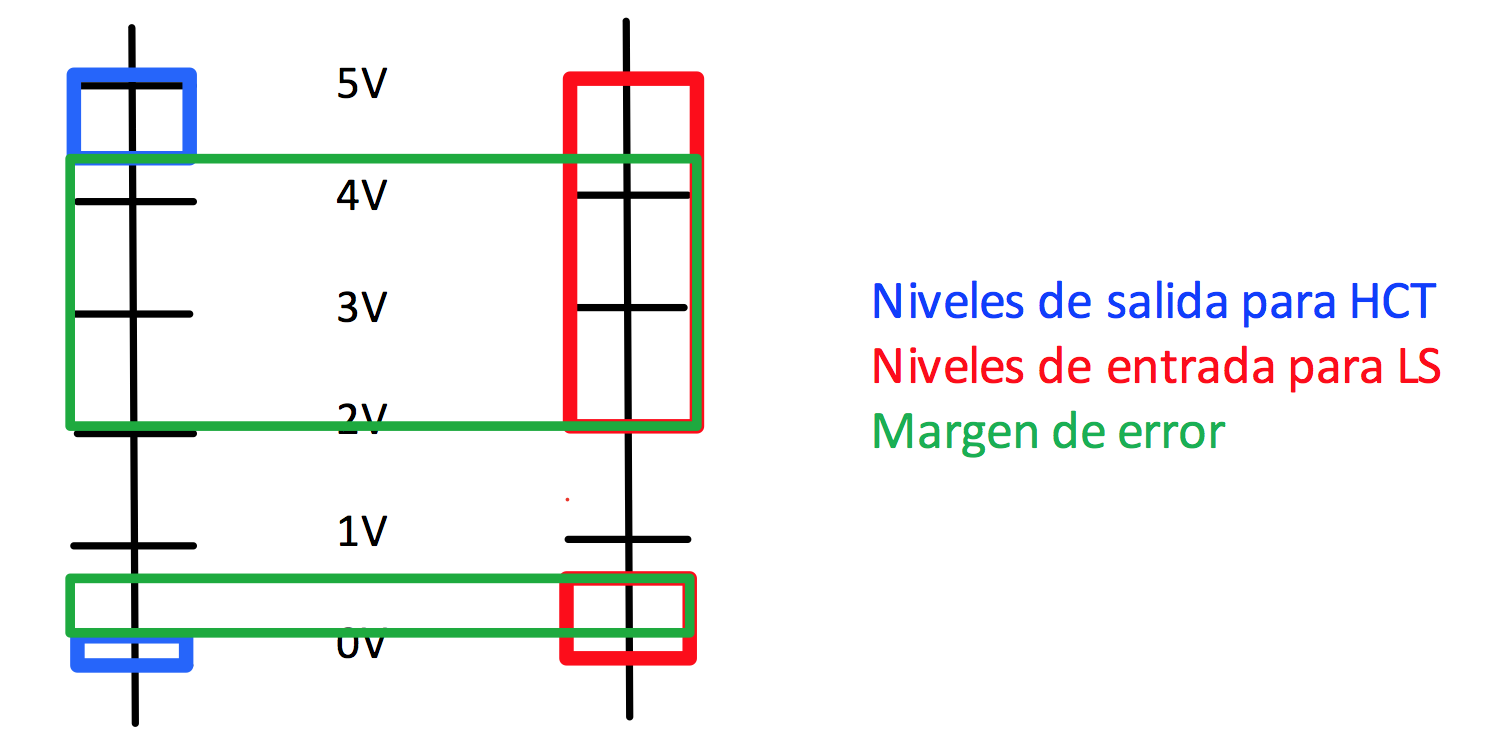
\includegraphics[width=6cm]{ejercicio2/HCT-LS}
    \caption{Niveles de tensi\'on para caso HCT alimenta a LS.} %caption abajo
  	\end{center}
  \caption{Circuito utilizado}
  \label{7_fig1}
  \end{minipage}
  \begin{minipage}[b]{0.4\textwidth}
    \begin{center}
  		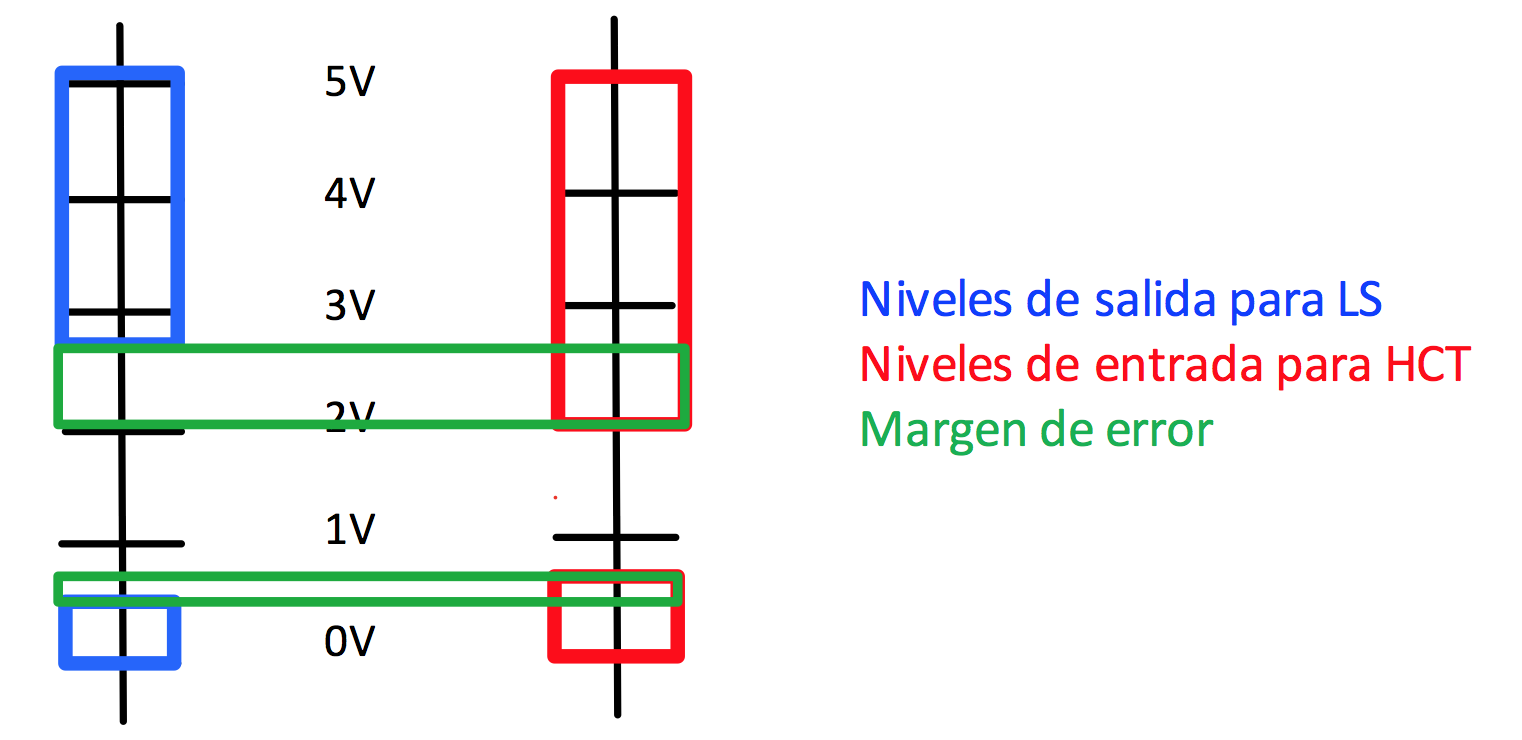
\includegraphics[width=6cm]{ejercicio2/LS-HCT}
    \caption{Niveles de tensi\'on para caso LS alimenta a HCT.} %caption abajo
	\end{center}
  \caption{Implementaci\'on con 74HC112}
  \label{7_fig2}
 \end{minipage}
\end{center}
\end{figure}


Procedimos a alimentar una compuerta del integrado LS02 con la salida de una misma compuerta pero del integrado HC02, y luego alimentamos de la misma manera pero en sentido inverso. Pudimos notar que hay zonas donde el circuito armado no deber\'ia andar de forma \'optima por el margen de ruido que manejan las distintas compuertas pero funciona igual ya que la ca\'ida de tensi\'on en el LS02 no es tan grande y alcanza a caer cerca del l\'imite del HC02 con 4,2V aproximadamente que es el m\'inimo del estado HIGH para el HC02. Si hubiera sido menor el valor de la tensi\'on no hubi\'eramos obtenido alguna salida por lo marcado en las hojas de datos.
\newline

El \textbf{fan-out} est\'a determinado por la cantidad de corriente que puede aceptar en la entrada cada CI y es la cantidad de pines que puede alimentar un CI con alguna de sus salidas. En la tecnolog\'ia CMOS(HC) seg\'un su hoja de dato acepta 20mA como m\'aximo, mientras que la tecnolog\'ia TTL(LS) acepta 0,4mA como m\'aximo en la entrada y 8mA en la salida. Haciendo las cuentas directas de estos casos, con la salida de un integrado LS puedo alimentar hasta 20 entradas LS, mientras que con un HC puedo alimentar 50 entradas LS. Cabe destacar que en la hoja de datos que brinda el fabricante solo asegura el funcionamiento de hasta 10 pines LS-TTL con una salida del HC, el cual debe ser para el peor caso que puede surgir para este integrado.
\newline

Al hacer las mediciones alimentando con el HCT y notamos un comportamiento mejor en cuanto la alimentaci\'on del LS02, ya que la tecnolog\'ia HCT es a base de CMOS pero tiene una gran tolerancia con la tecnolog\'ia TTL en cuanto a los valores de tensi\'on.
\newline
\textbf{OBSERVACI\'ON:} Haciendo zoom en las señales se puede observar que la tecnolog\'ia TTL siempre otorga una tensi\'on m\'as baja de lo esperado, esto se debe a que internamente contiene una resistencia que l\'imita la corriente que circular\'a por el transistor pero provocar\'a una ca\'ida de tensi\'on la cual se ve reflejada a la salida. Por otra parte la tecnolog\'ia CMOS tiene un efecto capacitivo interno que provoca una pequeña oscilaci\'on cuando responde al escal\'on. Aqu\'i dejamos unas imagenes mostrando los efectos mencionados.

\begin{figure}[H]
\begin{center}
  \begin{minipage}[b]{0.4\textwidth}
  	\begin{center}
  		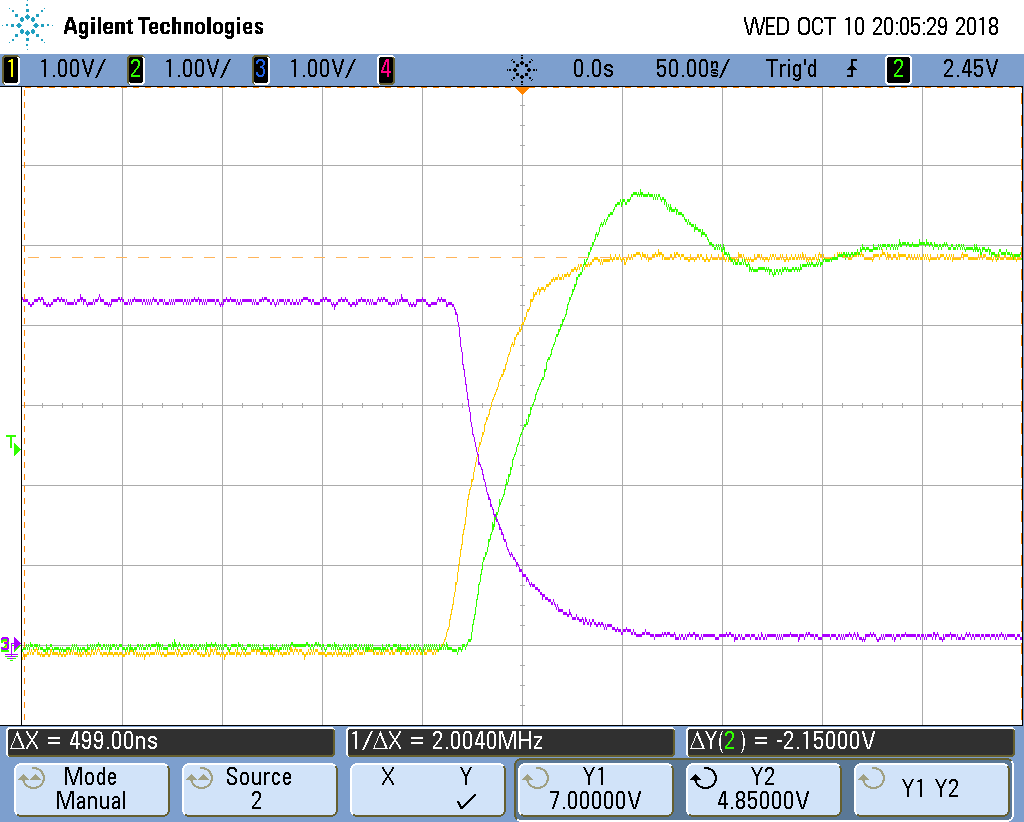
\includegraphics[width=6cm]{ejercicio2/OSC_LS_HC.png}
		\caption{LS alimentando al HC}
  	\end{center}
  \caption{Circuito utilizado}
  \label{7_fig1}
  \end{minipage}
  \begin{minipage}[b]{0.4\textwidth}
    \begin{center}
  		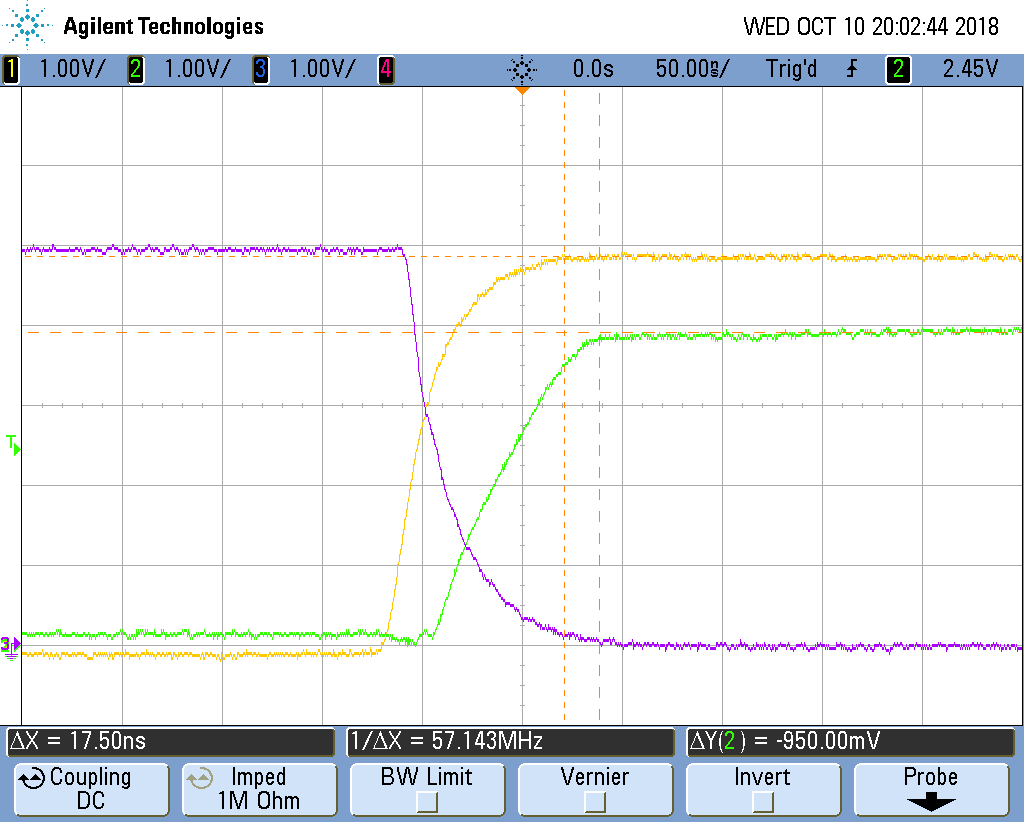
\includegraphics[width=6cm]{ejercicio2/OSC_HC_LS.png}
		\caption{HC alimentando al LS}
	\end{center}
  \caption{Implementaci\'on con 74HC112}
  \label{7_fig2}
 \end{minipage}
\end{center}
\end{figure}

\begin{figure}[hbtp]
	\centering
		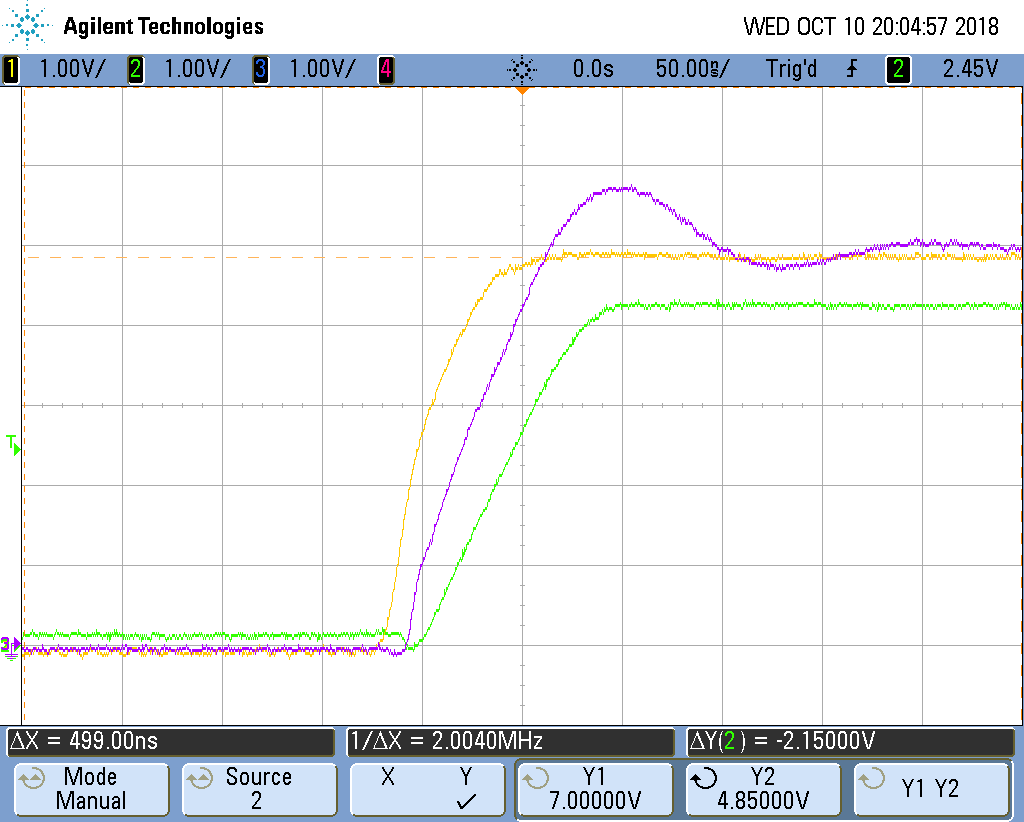
\includegraphics[width=8cm]{ejercicio2/OSC_AMBAS.png}
	\caption{Ambas señales sobrepuestas}
\end{figure}

En las im\'agenes anteriores la señal amarilla es la de entrada, la cual corresponde a una onda cuadrada que va de 0V a 5V. La señal verde es la de salida y la violeta es la señal intermedia (la señal que esta entre compuerta y compuerta). Mientras que en la tercer im\'agen est\'an sobrepuestas ambas señales de salida, donde la amarilla corresponde a la de entrada, la señal verde a la salida del 74LS02 y la señal violeta es la salida del 74HC02.



